\section{Government}
	\subsection{Registration}
	The government cannot register a new account like citizens and 
	businesses because only one account is allowed. This account is provided 
	by the developer of \textit{Soldino}.
	\subsection{Login}
	If you want to log on the Government account press the "login" button on the 
	top right of the homepage, you will automatically log in your account 
	(there is no need for a username or password, all is done via MetaMask). 
	\\To be able to log in make sure you are logged in the correct MetaMask\glosp 
	account.
	\subsection{Logout}
	To log out of \textit{Soldino} you just have to log out of 
	MetaMask\glosp. To do this you have to press MetaMask's icon on the top 
	right of the browser, press your account's icon and then press "Log out"
	on the top right.
	\begin{figure}[H]
		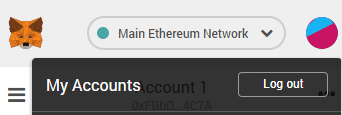
\includegraphics[width=7cm]{res/images/logout_metamask.png}
		\centering
		\caption{Logging out}
	\end{figure}
	\subsection{Cubit}
		\subsubsection{Minting}
		The Government can mint Cubits\glo. This can be done by visiting the dedicated page, you can find the "Cubit Manager" button in the navigation bar at the top of the page.
%		
		\subsubsection{Distributing}
		The Government can distribute Cubits\glosp previously minted amongst the users 
		of the platform. This can be done by visiting the dedicated page, you can find the "Cubit Manager" button in the navigation bar at the top of the page.
%		
	\subsection{Managing users}
	The Government can activate disabled accounts or deactivate active accounts.
	This can be done by visiting the page containing all users registered on the
	platform, clicking on the "Users List" button in the navigation bar at the top of the page.
%	
		\subsubsection{Activating users}
		After you have found the account you want to enable press the button 
		"Enable". After being enabled an account will again be able to make 
		purchases on \textit{Soldino}.
%		
		\subsubsection{Deactivating users}
		After you have found the account you want to disable press the 
		"Disable" button. After pressing it a window will open where you can 
		write a	message explaining why the account was disabled that will be 
		shown when that user will try an log in. Disabling an account 
		means that it will not be able to make purchases on \textit{Soldino} 
		until it is enabled.
%		
	\subsection{Reimbursing businesses}
	The Government can reimburse business of their VAT credit. This can be done 
	by doing click on the "VAT Refund" button in the navigation bat at the top of the page.
%	